\documentclass[dvipdfmx,b5paper]{jsarticle}

\usepackage{amsmath,amssymb}
\usepackage{amsthm}
\usepackage{bm}
\usepackage[dvipdfmx]{graphicx}
\usepackage{ascmac}
\usepackage{subfigure}
\usepackage{verbatim}
\usepackage{wrapfig}
\usepackage{makeidx}
\usepackage[dvipdfmx]{hyperref}
\usepackage{setspace}
\usepackage{color}
\usepackage{listings}
\usepackage{tikz}
\usepackage{otf}
\usepackage{multirow}
\usetikzlibrary{intersections, calc, arrows}
\usetikzlibrary{decorations,decorations.pathmorphing}
\usepackage{cleveref}
\usepackage{mathtools}

\usepackage{framed}
\usepackage{here}
\usepackage{pdfpages}

\usepackage{siunitx}
\usepackage{here}

\usepackage{bm}

\newcommand{\oover}[1]{\overline{\overline{#1}}}

% \usepackage{listings, jlisting, color}
% \definecolor{OliveGreen}{rgb}{0.0,0.6,0.0}
% \definecolor{Orenge}{rgb}{0.89,0.55,0}
% \definecolor{SkyBlue}{rgb}{0.28, 0.28, 0.95}
% \lstset{
%   language={C}, % 言語の指定
%   basicstyle={\ttfamily},
%   identifierstyle={\small},
%   commentstyle={\smallitshape},
%   keywordstyle={\small\bfseries},
%   ndkeywordstyle={\small},
%   stringstyle={\small\ttfamily},
%   frame={tb},
%   breaklines=true,
%   columns=[l]{fullflexible},
%   numbers=left,
%   xrightmargin=0zw,
%   xleftmargin=3zw,
%   numberstyle={\scriptsize},
%   stepnumber=1,
%   numbersep=1zw,
%   lineskip=-0.5ex,
%   keywordstyle={\color{SkyBlue}},     %キーワード(int, ifなど)の書体指定
%   commentstyle={\color{OliveGreen}},  %注釈の書体
%   stringstyle=\color{Orenge}          %文字列
% }

\usepackage{listings, xcolor}

\lstset{
    basicstyle = {\ttfamily}, % 基本的なフォントスタイル
    frame = {tbrl}, % 枠線の枠線。t: top, b: bottom, r: right, l: left
    breaklines = true, % 長い行の改行
    numbers = left, % 行番号の表示。left, right, none
    showspaces = false, % スペースの表示
    showstringspaces = false, % 文字列中のスペースの表示
    showtabs = false, % タブの表示
    keywordstyle = \color{blue}, % キーワードのスタイル。intやwhileなど
    commentstyle = {\color[HTML]{1AB91A}}, % コメントのスタイル
    identifierstyle = \color{black}, % 識別子のスタイル 関数名や変数名
    stringstyle = \color{brown}, % 文字列のスタイル
    captionpos = t % キャプションの位置 t: 上、b: 下
}

\title{課題演習C1 最終レポート}
\author{0500-34-0042 \quad 大平 達也}
\date{\today}

\begin{document}
\maketitle

\section{はじめに}
本稿では, 課題演習C1のまとめとして, 磁場なしの衝撃波管問題を通して数値計算の手法について概観していく。

\section{問題設定・目的}
衝撃波管問題は, 物理量$\bm{U}$が初期に不連続を持つときの, 1次元Euler方程式の解を求める問題である。より具体的には, 図\ref{shocktube}のように, 十分に長い, 仕切られた管の片側に高圧の, もう片側に低圧の流体をいれ, 仕切りを取り去ることで衝撃波等が発生することがある, というものである。

\begin{figure}[H]
\centering
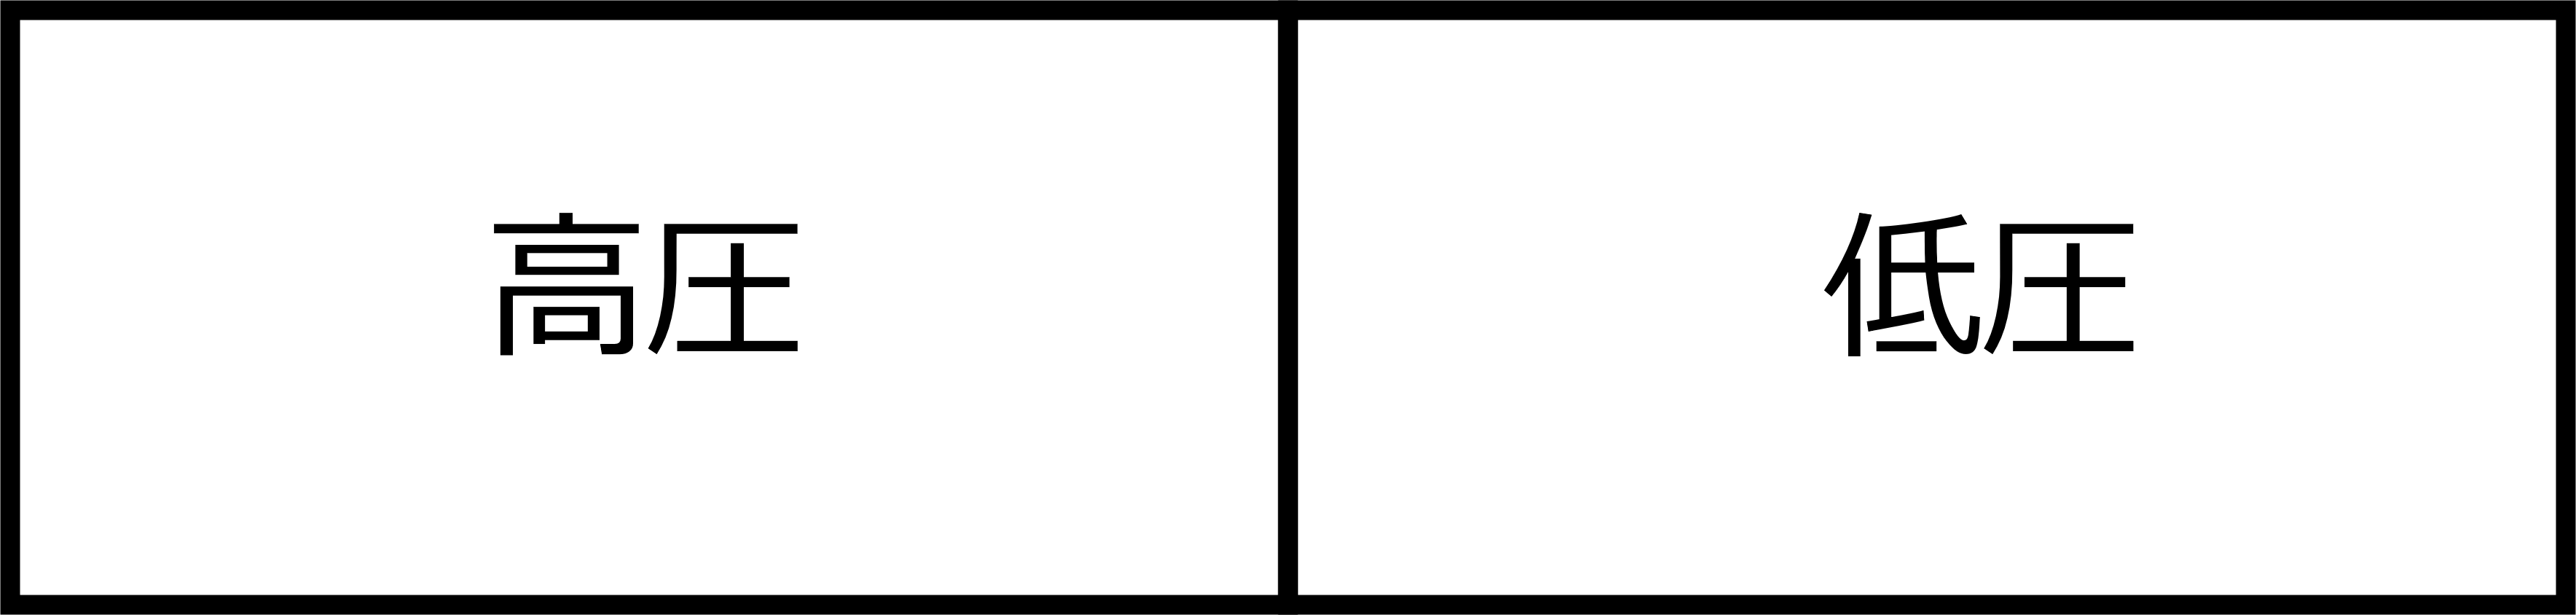
\includegraphics[width=0.4\linewidth]{fig/shocktube.png}
\caption{衝撃波管問題のイメージ図}
\label{shocktube}
\end{figure}

\section{物理的背景}
\subsection{設定について}
簡単のため, ここで扱う流体は非粘性・圧縮流体を仮定する。また, 管に沿った方向以外の方向での流体の速度はゼロであると仮定する。扱う基礎方程式を記す: 
\begin{equation}
  \frac{\partial}{\partial t}\rho+\frac{\partial}{\partial x}(\rho u)=0
\end{equation}
\begin{equation}
  \frac{\partial}{\partial t}(\rho u)+\frac{\partial}{\partial x}(rho u^2+p)=0
\end{equation}
\begin{equation}
  \frac{\partial}{\partial t}\left[\frac{p}{\gamma-1}+\frac{1}{2}\rho u^2\right]+\frac{\partial}{\partial x}\left[\left(\frac{\gamma}{\gamma-1}p+\frac{1}{2}\rho u^2\right)u\right]=0
\end{equation}

上から順に, 連続の式, 運動量保存則, エネルギー保存則を表す。

ただし, 以下では, これと同値である, 1つにまとめた次の形を用いることがある: 
\begin{equation}
  \frac{\partial \bm{U}}{\partial t}+\frac{\partial \bm{F}}{\partial x}=0
  \label{eq}
\end{equation}

ただし, 
\begin{equation}
  \bm{U}=
  \begin{pmatrix}
    \rho \\
    \rho v \\
    \rho E
  \end{pmatrix}, 
\end{equation}
\begin{equation}
  \bm{F}=
  \begin{pmatrix}
    \rho v \\
    \rho v^2+p \\
    \rho \rho Hv
  \end{pmatrix}.  
\end{equation}
である。ここで, $H=E+\frac{p}{\rho}$は単位質量あたりのエンタルピーとした。

また, 初期条件について, 初期での不連続点は原点$x=0$にあるとし, 初期条件を次のように書くこととする: 
\begin{eqnarray*}
  \bm{U}(x, 0)=
    \begin{cases}
        \bm{U}_{\mathrm{L}}\quad (x<0), \\
        \bm{U}_{\mathrm{R}}\quad (x\geq 0). 
    \end{cases}
\end{eqnarray*}

\subsection{現象の説明}

数値解の一例を図\ref{ex}に示す。この通り, 3つの急激な値の変化がみられる。これは左から, 膨張波, 接触不連続面, 衝撃波である。接触不連続面は, 密度は不連続であるものの, 圧力と速度が連続的に接している面であり, この面を境として温度が異なるガスが圧力平衡で接している。

\begin{figure}[H]
  \centering
  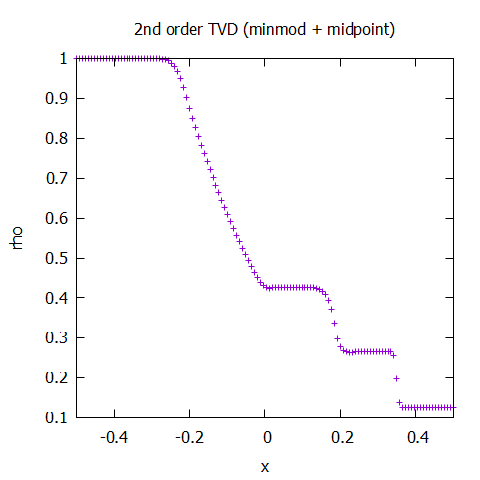
\includegraphics[width = 0.6\linewidth]{../book/chap03/10_shock-tube-minmod/03.png}
  \caption{衝撃波管問題の数値解の一例}
  \label{ex}
\end{figure}

\section{実装の方針}
\subsection{Riemann fanについて}
衝撃波管問題の解は, 衝撃波, 接触不連続面, 膨張波の組み合わせで構成され, 衝撃波, 接触不連続面, 膨張波はそれぞれ一定の速度で空間を伝播する。そのため, ある時刻の衝撃波管問題の解は, 別の時刻の解と相似的になっている。すなわち, $x-t$空間を考えると, 衝撃波, 接触不連続面, 膨張波の軌跡は原点から放射状に広がる。これをRiemann fanという (図\ref{fan}参照)。

\begin{figure}[H]
  \centering
  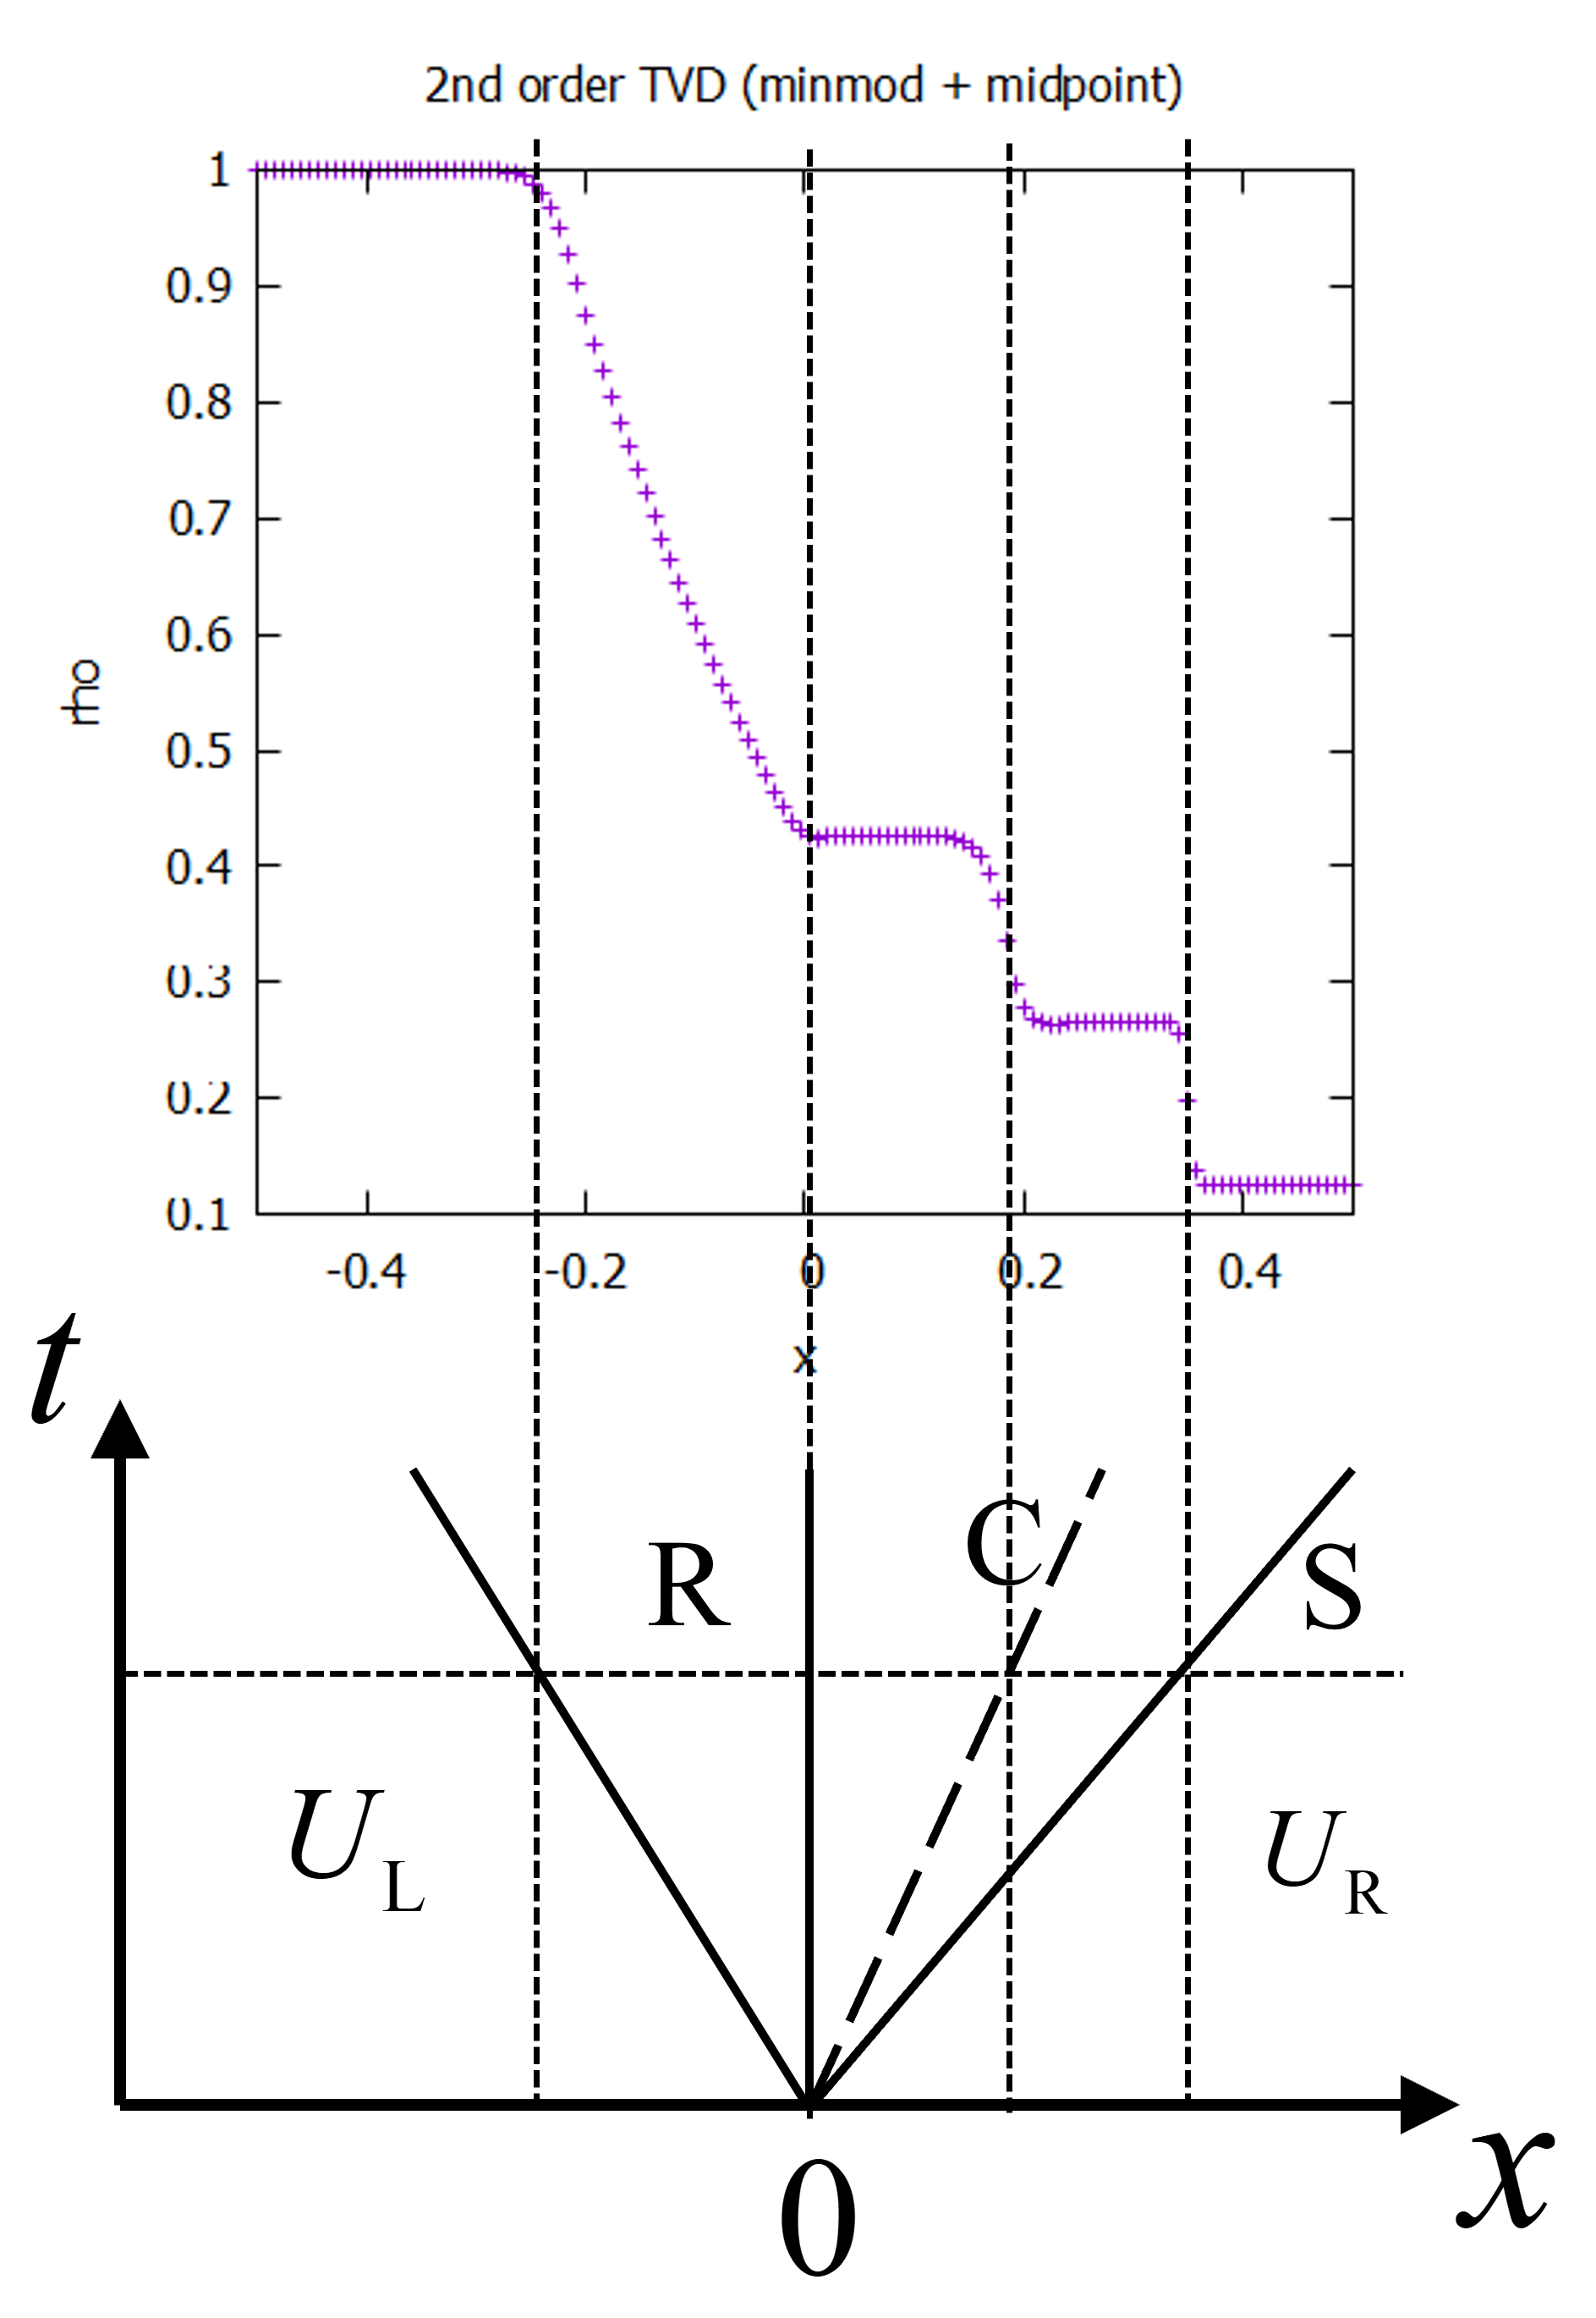
\includegraphics[width = 0.6\linewidth]{fig/riemannfan.png}
  \caption{Riemann fan}
  \label{fan}
\end{figure}

\subsection{有限体積法}
まず, 今回数値計算を行う上で基本となる有限体積法を導出する。

Euler方程式(\refeq{eq})をセルの区間$x_{i-1/2}\leq x\leq x_{i+1/2}$において$x$で積分し, 時間刻みの区間$t_n\leq t\leq t_{n+1}$において積分する。その結果, 
\begin{equation}
  \bm{U}_{i}^{n+1}=\bm{U}_{i}^{n}-\frac{\Delta t}{\Delta x}\left(\overline{\bm{F}}_{i+1/2}-\overline{\bm{F}}_{i-1/2}\right)
\end{equation}
となる。ここで, 時刻$t=t_n$におけるセル$i$内部の$\bm{U}$の平均値を
\begin{equation}
  \bm{U}_{i}^{n}=\frac{1}{\Delta x}\int_{x_{i-1/2}}^{x_{i+1/2}}\bm{U}(x, t_n)dx
\end{equation}
と定義した。また, セル境界$x=x_{i+1/2}$における時間区間$t_n\leq t\leq t_{n+1}$の流束$\bm{F}$の平均値を, 
\begin{equation}
  \overline{\bm{F}}_{i+1/2}=\frac{1}{\Delta t}\int_{t_{n}}^{t_{n+1}}\bm{F}(\bm{U}(x_{i+1/2}, t))dt
\end{equation}
と定義する。

\subsection{Godnov法}
前項で出てきた数値流束をどのように求めるかについて考えていく。

今回衝撃波管問題を解くのに用いたスキームは, Godnovスキームと呼ばれるものである。この節では, Godnovスキームについて概説する。

まず, 衝撃波管問題の解は, 左右の物理量の関数になっているため, 衝撃波管問題の解を
\begin{equation}
  \bm{U}(x, t)=\mathcal{RP}\left(\frac{x}{t}, \bm{U}_{\mathrm{L}}, \bm{U}_{\mathrm{R}}\right)
\end{equation}
と書くことができる。以下, $\mathcal{RP}$を衝撃波管問題の解を返す関数として, この記法を用いる。

セル内の物理量$U$が一定であるというのは, 有限体積法の考え方である。この考えのため, セル境界$i+1/2$に不連続があると考えることができる。この不連続面において, 衝撃波管問題を考える。ここで, 時間刻み$\Delta t$の間に$U$が衝撃波管問題の解に従って変化し, 時間ステップの最後にセル内部の物理量$U$を平均化することで, 区分的に一定の関数$\bm{U}_{i}^{n+1}$を求めるとすればよい。これがGodnov法である。

このとき流束は, 
\begin{equation}
  \overline{\bm{F}}_{i+1/2}=\frac{1}{\Delta t}\int_{t_{n}}^{t_{n+1}}\bm{F}(\mathcal{RP}(0, \bm{U}_{i}^{n}, \bm{U}_{i}^{n+1}))dt
  \label{flux_calc}
\end{equation}
とかける\footnote{ここで, セル境界$x=x_{i+1/2}$において衝撃波管問題を解くため, 第1変数はゼロになっている}。
この関数$\mathcal{RP}(0, \bm{U}_{i}^{n}, \bm{U}_{i}^{n+1})$は時間的に一定であるため, \refeq{flux_calc}は, 
\begin{equation}
  \bm{F}_{I+1/2}^{*\mathrm{(Godnov)}}=\bm{F}(\mathcal{RP}(0, \bm{U}_{i}^{n}, \bm{U}_{i}^{n+1}))
\end{equation}
となる。これがGodnov法の数値流束である。

\subsection{Roeの方法}

前節で, Godnov法の数値流束について議論した。この説では, この数値流束の具体的な求め方について議論し, Roeの方法を説明する。

通常のGodnov法においては, 数値流束を求める際に衝撃波管問題の解として厳密解を用いる。しかし, 衝撃波管問題の厳密解を求めるには, 反復法を用いる必要があり, 計算コストが高い。そのため, 衝撃波管問題の近似解を用いることを考える。この近似解を求める方法として, 今回はRoeの方法を採用した。

まず, 流束は保存変数の関数として, 
\begin{equation}
  \bm{F}=\bm{F}(\bm{U})
\end{equation}
とかけるため, \refeq{eq}を次のように変形する: 
\begin{equation}
  \frac{\partial \bm{U}}{\partial t}+\bm{A}\frac{\partial \bm{U}}{\partial x}=0
  \label{eqneo}
\end{equation}
ここで, $\bm{A}$はJacobi行列で, 
\begin{equation}
  \bm{A}=\frac{\partial \bm{F}}{\partial \bm{U}}=
  \begin{pmatrix}
    0 & 1 & 0 \\
    -(3-\gamma_{\mathrm{ad}})\frac{v^2}{2} & (3-\gamma_{\mathrm{ad}})v & \gamma_{\mathrm{ad}}-1 \\
    -Hv+(\gamma_{\mathrm{ad}}-1)\frac{v^3}{2} & H-(\gamma_{\mathrm{ad}}-1)v^2 & \gamma_{\mathrm{ad}}v
  \end{pmatrix}
\end{equation}
である。

$\bm{A}$を対角化しておく。固有値$\lambda$は, 
\begin{equation}
  \lambda_1=v-c_s, \lambda_2=v, \lambda_3=v+c_s
\end{equation}

右固有行列$\bm{R}$を, 
\begin{equation}
  \bm{R} = 
  \begin{pmatrix}
    \bm{r}^{(1)} & \bm{r}^{(2)} & \bm{r}^{(3)}
  \end{pmatrix}
  =
  \begin{pmatrix}
    1 & 1 & 1 \\
    v-c_s & v & v+c_s \\
    H-vc_s & \frac{v^2}{2} & H+vc_s
  \end{pmatrix}
\end{equation}
とする。これの逆行列を計算すると, 
\begin{equation}
  \bm{R}^{-1}=
  \begin{pmatrix}
    \frac{1}{2}\left(b_1+\frac{v}{c_s}\right) & -\frac{1}{2}\left(\frac{1}{c_s}+b_2v\right) & \frac{1}{2}b_2 \\
    1-b_1 & b_2v & -b_2 \\
    \frac{1}{2}\left(b_1-\frac{v}{c_s}\right) & \frac{1}{2}\left(\frac{1}{c_s}-b_2v\right) & \frac{1}{2}b_2
  \end{pmatrix}
\end{equation}
となり, これを$\bm{L}$と定義する。ただし, 
\begin{equation}
  b_1=\frac{\gamma_{\mathrm{ad}}-1}{c_s^2}\frac{v^2}{2}, b_2=\frac{\gamma_{\mathrm{ad}}-1}{c_s^2}
\end{equation}
とする。$\bm{R}, \bm{L}$より, $\bm{A}$が, 
\begin{equation}
  \bm{\Lambda}=\bm{LAR}
\end{equation}
と対角化できた。ただし, 
\begin{equation}
  \bm{\Lambda}=
  \begin{pmatrix}
    \lambda_1 & 0 & 0 \\
    0 & \lambda_2 & 0 \\
    0 & 0 & \lambda_3
  \end{pmatrix}
\end{equation}
である。

物理量は, セル境界を挟んで微小な変位$\delta \bm{U}=\bm{U}_{i+1}-\bm{U}_{i}$を持つが, \refeq{eqneo}において行列$\bm{A}$は一定であると近似する\footnote{線形近似である}。$\bm{A}$が変わらないため, 固有値$\lambda_j$や$\bm{L}, \bm{R}$も一定である。

ここで, 変位$\delta \bm{U}$について, 新しい変数$\partial \bm{W}=(\partial w_1, \partial w_2, \partial w_3)^{\mathrm{T}}=\bm{L}\delta\bm{U}$を考える。各成分は, 
\begin{equation}
  \partial w_1=\frac{\rho}{2c_s}\left(\frac{\delta p}{\rho c_s}-\delta v\right)
\end{equation}
\begin{equation}
  \partial w_2 = \delta \rho-\frac{\delta p}{c_s^2}
\end{equation}
\begin{equation}
  \partial w_3 = \frac{\rho}{2c_s}\left(\frac{\delta p}{\rho c_s}+\delta v\right)
\end{equation}

次に, Euler方程式\refeq{eqneo}の第2項を離散化する。
\begin{eqnarray}
  \bm{A}\left(\frac{\partial \bm{U}}{\partial x}\right)^{\mathrm{(uw)}} &=& \bm{R}(\bm{LAR})\bm{L}\left(\frac{\partial \bm{U}}{\partial x}\right)^{\mathrm{(uw)}} \\
  &=& \bm{R\Lambda}\left(\frac{\partial \bm{W}}{\partial x}\right)^{\mathrm{(uw)}} \\
  &=& \begin{pmatrix}
    \bm{r}^{(1)} & \bm{r}^{(2)} & \bm{r}^{(3)}
  \end{pmatrix}
  \begin{pmatrix}
    \lambda_1 & 0 & 0 \\
    0 & \lambda_2 & 0 \\
    0 & 0 & \lambda_3
  \end{pmatrix}
  \begin{pmatrix}
    \partial w_1/\partial x \\
    \partial w_2/\partial x \\
    \partial w_3/\partial x 
  \end{pmatrix}^{\mathrm{(uw)}} \\
  &=& \sum_{j=1}^{3}\lambda_j\left(\frac{\partial w_j}{\partial x}\right)^{\mathrm{uw}}\bm{r}^{(j)}
\end{eqnarray}
となる。

すなわち, Euler方程式を固有ベクトル$\bm{r}^{\mathrm{(j)}}$を用いて展開すると, $\partial w_j$に関する3つのスカラー線形波動方程式の重ね合わせとして書けることが分かった。

よって, それぞれの波について風上差分で評価すればよく, 数値流束は, 
\begin{equation}
  \bm{F}_{i+1/2}^{*}=\frac{1}{2}\left(\bm{F}_{i}+\bm{F}_{i+1}\right)-\frac{1}{2}\sum_{j=1}^{3}|\lambda_j|\partial w_j\bm{r}^{(j)}
  \label{flux_liner}
\end{equation}
となる。

ここから, \refeq{flux_liner}を非線形に拡張することを考える。すなわち, $\delta\bm{U}$が有限の大きさのとき, セル境界における行列$\bm{A}_{i+1/2}$をどのように与えるかについて考えなければならない。

$\bm{A}$は次の3つの性質を満たす行列$\oover{\bm{A}}$であるべきである。
\begin{itemize}
  \item 物理量$\bm{U}_{i}$, $\bm{U}_{i+1}$について, 
  \begin{equation}
    \bm{F}_{i+1}-\bm{F}_{i} = \oover{\bm{A}}(\bm{U}_{i}, \bm{U}_{i+1})(\bm{U}_{i}-\bm{U}_{i+1})
  \end{equation}
  が成立すること。
  \item 左右の物理量が等しいとき ($\bm{U}_{i}=\bm{U}_{i+1}=\bm{U}$), 
  \begin{equation}
    \oover{\bm{A}}(\bm{U}, \bm{U})=\bm{A}(\bm{U})\equiv\frac{\partial \bm{F}}{\partial \bm{U}}
  \end{equation}
  が成立すること。
  \item 行列$\oover{\bm{A}}$が実数の固有値と線形独立な固有ベクトルを持つこと。
\end{itemize}
$\oover{\bm{A}}$がこの3条件を満たせば, 線形の場合の議論がそのまま非線形の場合に用いることができる。

$\bm{A}$に現れる$\rho, v, H$を, 次で定義される$\oover{\rho}, \oover{v}, \oover{H}$に置き換えて$\oover{A}$を計算すると, この3条件を満たす。
\begin{equation}
  \oover{\rho}_{i+1/2}=\sqrt{\rho_{i}\rho_{i+1}}
\end{equation}
\begin{equation}
  \oover{v}_{1+1/2}=\frac{v_i\sqrt{\rho_i}+v_{i+1}\sqrt{\rho_{i+1}}}{\sqrt{\rho_i}+\sqrt{\rho_{i+1}}}
\end{equation}
\begin{equation}
  \oover{H}_{1+1/2}=\frac{H_i\sqrt{\rho_i}+H_{i+1}\sqrt{\rho_{i+1}}}{\sqrt{\rho_i}+\sqrt{\rho_{i+1}}}
\end{equation}

これがRoeの方法である。

\section{実装}
コードを以下に記す。
\lstinputlisting[caption=衝撃波管問題 (Roeの方法), label=code:roe, language=C]{../book/chap03/01_roe-1/01.c}

\section{実行結果}

上記コードを実行したのち, gnuplotで可視化した図を以下に示す。
\begin{figure}[H]
  \centering
  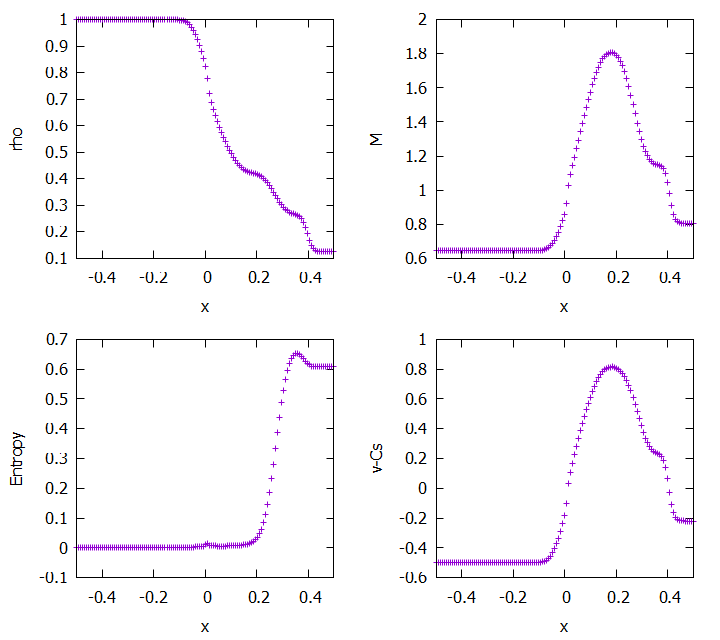
\includegraphics[width = 0.8\linewidth]{../book/chap03/01_roe-1/out/01-2-2.png}
  \caption{衝撃波管問題をRoeの方法で解いたplot}
  \label{fig:roe}
\end{figure}

全体的になまった解ではあるが, 衝撃波と接触不連続面については安定に解けている。しかし, 膨張波について不連続が発生している。これは, 膨張衝撃波と呼ばれる, 現実には存在しない解である。これの対処について次の節で述べる。

\section{エントロピー補正}
通常の衝撃波では, 流体は衝撃波に対して超音速で流入し, 亜音速で流出し, その際に流体の運動エネルギーが熱エネルギーに変換される。この状況を時間反転した状態を考えると, エントロピーが減少してしまい, 物理的にありえない。これが膨張衝撃波である。

膨張衝撃波を抑制する方法として, エントロピー補正を考える。不連続面で波の速度がゼロにならないように補正する。そのため, Roeの数値流束に現れる$|\oover{\lambda}|_{i+1/2}$を次の$|\oover{\lambda}|_{\mathrm{mod}}$に置き換えて, 波の速度を補正する。この方法は膨張波において数値粘性を多めに加えることで膨張衝撃波をなまらせる方法であると考えることもできる。
\begin{eqnarray*}
  |\oover{\lambda}|_{\mathrm{mod}}=
    \begin{cases}
      |\oover{\lambda}|_{i+1/2}\quad (|\oover{\lambda}|_{i+1/2}\geq\epsilon), \\
      \frac{1}{2}\left(\frac{\oover{\lambda}_{i+1/2}^2}{\epsilon}+\epsilon\right)\quad (|\oover{\lambda}|_{i+1/2}<\epsilon). 
    \end{cases}
\end{eqnarray*}
\begin{equation}
  \epsilon=\max[0, \oover{\lambda}_{i+1/2}-\lambda_i, \lambda_{i+1}-\oover{\lambda}_{i+1/2}]
\end{equation}

これを用いてplotした結果を次に示す。
\begin{figure}[H]
  \centering
  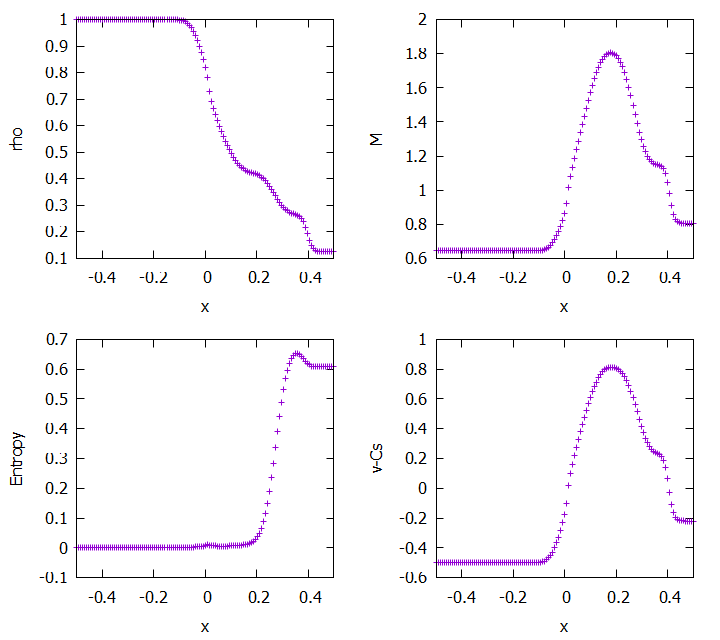
\includegraphics[width = 0.8\linewidth]{../book/chap03/02_entropy-modify/out/01.png}
  \caption{エントロピー補正したときのplot}
  \label{fig:entropy}
\end{figure}

\section{高次元化}
まず空間2次元の手法としてMUSCLを用いた。そこに制限関数を後で導入する。
次に時間についても2次元にしたい。本稿では中点法とHeun法を用いる。
\subsection{MUSCL}
区間$x_{i-1/2}<x<x_{i+1/2}$内で, 物理量を次のように展開する: 
\begin{equation}
  u(x)=u_i+(x-x_i)\left(\frac{\partial u}{\partial x}\right)_{i}+\frac{3\kappa}{2}\left[(x-x_i)^2-\frac{(\Delta x)^2}{12}\right]\left(\frac{\partial^2 u}{\partial x^2}\right)_{i}
  \label{muscl}
\end{equation}
ここで, $u_i$はセル内の平均値とする。$\kappa=1/3$のとき, \refeq{muscl}はTaylor展開に2次まで一致するため, 3次精度になる。$\kappa\neq1/3$のときは2次精度となる。

数値流束を求める際に, セル境界の値が必要になる。これまではセル内の値を一定として数値流束を計算したが, MUSCLでは\refeq{muscl}をにより, より近い値を補間し, それを用いることで高次元化を実現する。

\subsection{制限関数}
MUSCLを用いたときに解が振動してしまうことがある。たとえば図\ref{limit}は, $\kappa=-1$としたときに, セル境界の値$u_{i+1/2}^{\mathrm{L}}$を求めようとしている状況である。

\begin{figure}[H]
  \centering
  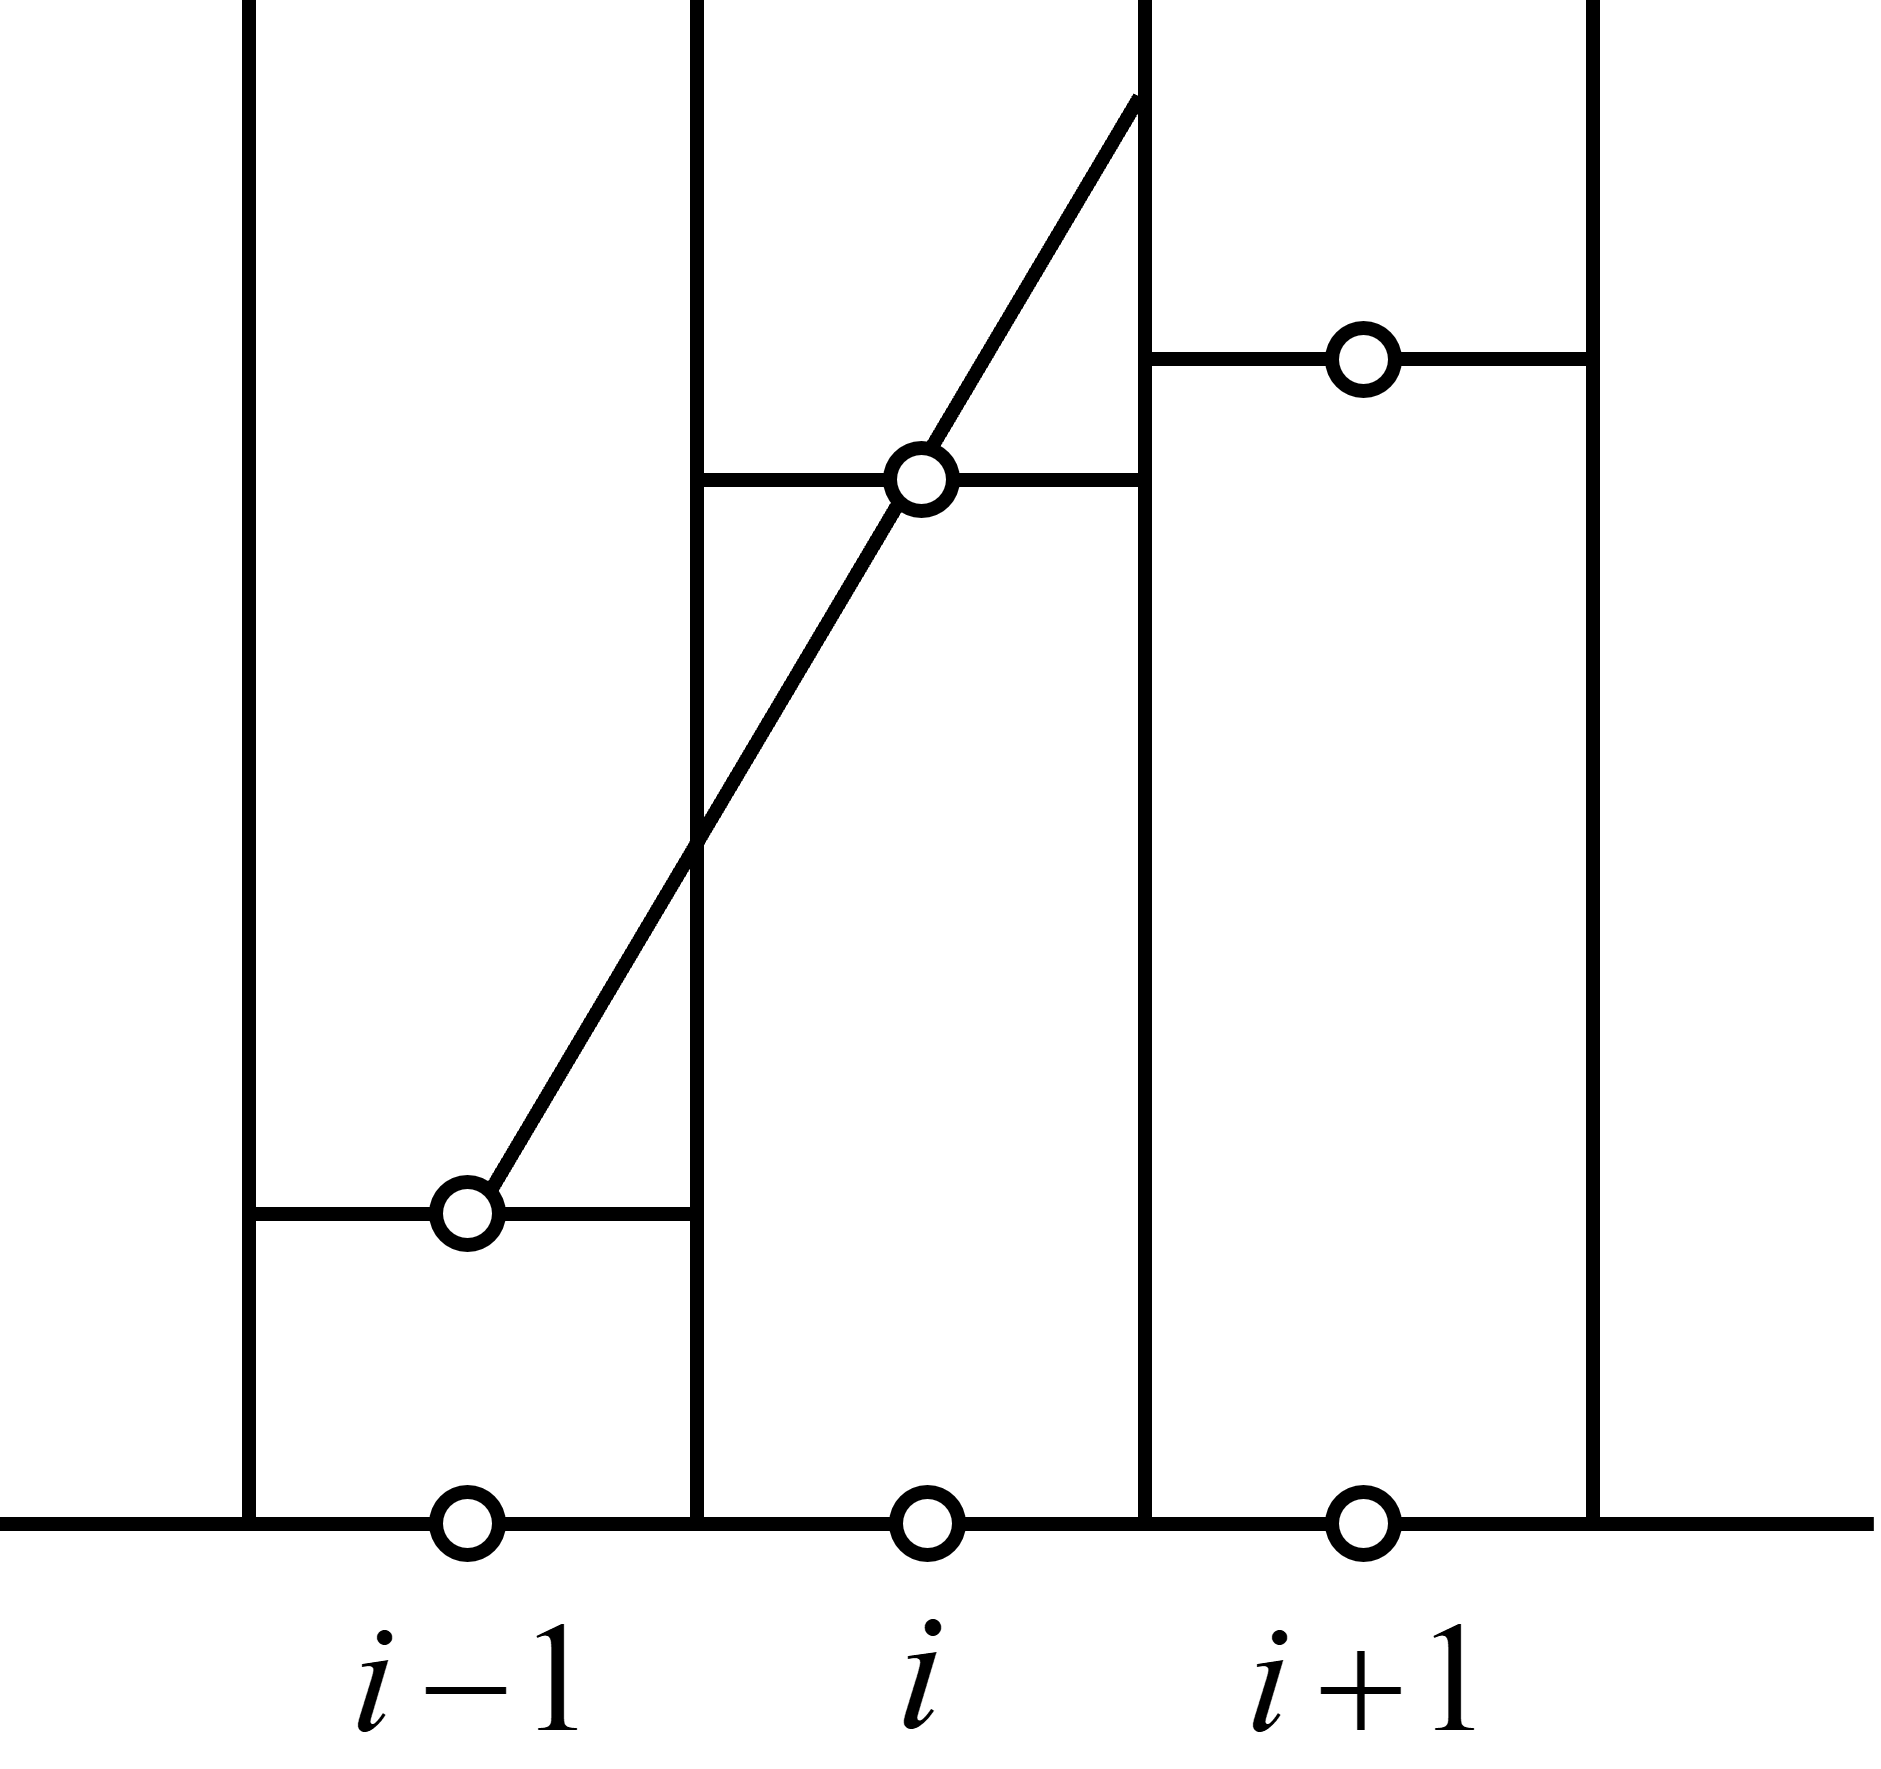
\includegraphics[width = 0.4\linewidth]{fig/limit.png}
  \caption{$u_{i-1}$と$u_i$を補間して$u_{i+1/2}^{\mathrm{L}}$を求める様子}
  \label{fig:limit}
\end{figure}

補間によって求められたセル境界の値は$u_{i+1/2}^{\mathrm{L}}>u_{i+1}$となり, 元の値の大小関係が逆転してしまっている。そのため, 勾配に制限をもうけることが必要である。

今回は, 制限関数として最も強いもの (superbee関数) と最も弱いもの (minmo
d関数) を用いて比較した。

ここで, minmod制限関数は, 
\begin{equation}
  \Psi(r)=minmod(r, 1)
\end{equation}
で, superbee関数は
\begin{equation}
  \Psi(r)=\max[0, \min(2r, 1), \min(r, 2)]
\end{equation}
で与えられる。

\subsection{実行結果と比較}
それぞれの制限関数用いて衝撃波管問題を解いた結果を以下の図に示す。

\begin{figure}[H]
  \centering
  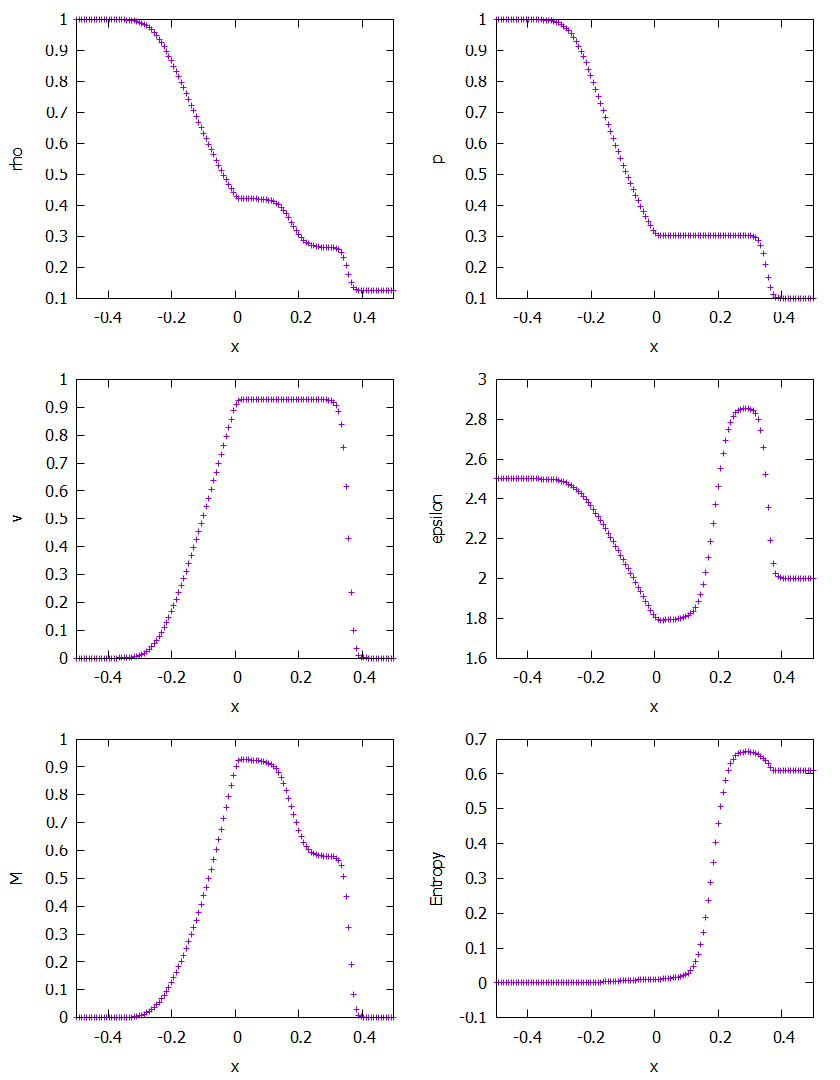
\includegraphics[width = 0.8\linewidth]{../book/chap03/10_shock-tube-minmod/01.png}
  \caption{衝撃波管問題をminmod制限関数を用いて解いたplot}
  \label{fig:minmod}
\end{figure}

\begin{figure}[H]
  \centering
  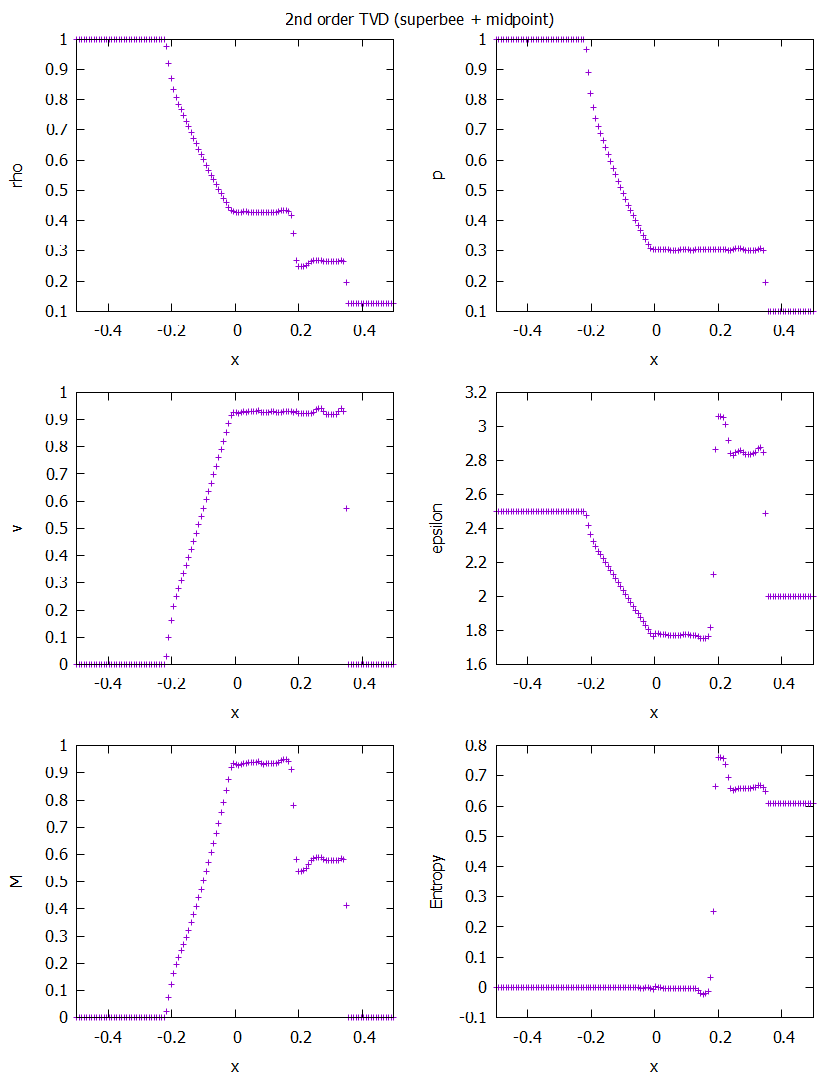
\includegraphics[width = 0.8\linewidth]{../book/chap03/11_shock-tude-superbee/01.png}
  \caption{衝撃波管問題をsuperbee制限関数を用いて解いたplot}
  \label{fig:superbee}
\end{figure}

この図の通り, (厳密解と比較しても) 2次精度において解の精度が上がっていることが確認された。また, より強いsuperbee制限関数を用いた場合のplotは, 全体的にシャープな印象を感じ, 特に接触不連続面と膨張波の部分において少ない点数で捉えれているように思った。しかし角が角張っている様子が見られた。この特徴は, 正弦波の線形移流方程式を解いた際にも見られたため, 矩形波を扱う分にはよいが, 多くの場合においてはminmod正弦関数が無難であるように考えられるが, 所々に物理量の振動が見られるため, 結局は精度自体をあげることがベストのように感じた。

\section{最後に・感想}
有名なテスト問題である衝撃波管問題を通して, 数値計算の様々な手法と考え方について学んだ。ただ, (HLL法は実装できたものの, ) 後半はHLLD法のバグをずっととれずに時間を費やしてしまい, 磁場ありの問題についてレポートをかくことができず, 非常に残念である。今回悔しい結果で終わってしまったため, 今後とも数値計算の勉強自体は続けれていければと思っている。

また, 本レポートでは省略した制限関数を用いて衝撃波管問題を解いた際のコードなど, C1で作成したほぼすべてのコードを, GitHubのPubric Repositryに格納してあるので, 参照いただけますと幸いです。

\url{https://github.com/mito-nya/c1_2024}

\begin{thebibliography}{9}
  \bibitem{matsumoto}
  松本倫明ほか. 輻射電磁流体シミュレーションの基礎. 日本評論社, 2024. 
  \bibitem{toro}
  Eleuterio F. Toro. Riemann Solvers and Numerical Method for Fluid Dynamics. Springer, 2009.
\end{thebibliography}
\end{document}